\subsubsection{Translação}

Se uma função real $g$ é tal que $g(x) = f(x+b) +a$, em que $f$ é outra função real e $b$ e $a$ são números reais,
então o gráfico de $g$ pode ser obtido, do gráfico de $f$, através
de uma translação horizontal de $\modu b$ unidades e uma
translação vertical de $\modu a$ unidades.
Os sinais de $a$ e $b$ influenciam nas translações vertical e horizontal, respectivamente, da seguinte forma:

\begin{itemize}
  \item $a > 0$: o translado vertical é no sentido positivo do eixo $y$ (para cima);
  \item $a < 0$: o translado vertical é no sentido negativo do eixo $y$ (para baixo);
  \item $b > 0$: o translado horizontal é no sentido negativo do eixo $x$ (para a esquerda);
  \item $b < 0$: o translado horizontal é no sentido positivo do eixo $x$ (para a direita).
\end{itemize}

\begin{example}
Sejam $f,g,h:\R \to \R$ tais que $f(x) = \sen x$, $g(x) = f(x) + 1 = \sen x +1$ e $h(x)= f\prn{x+\frac {\pi} 2}= \sen \prn{x+ \frac {\pi} 2}$.
Compare os gráficos de $h$ e $g$ ao gráfico de $f$ com relação a translações.
\end{example}

\begin{solution}
Na Imagem~\ref{img:grafico-translacao-exemplo-g}, é mostrado o gráfico de $g$.
%
  \begin{figure}
    \centering
    

\tikzset{every picture/.style={line width=0.75pt}} %set default line width to 0.75pt        

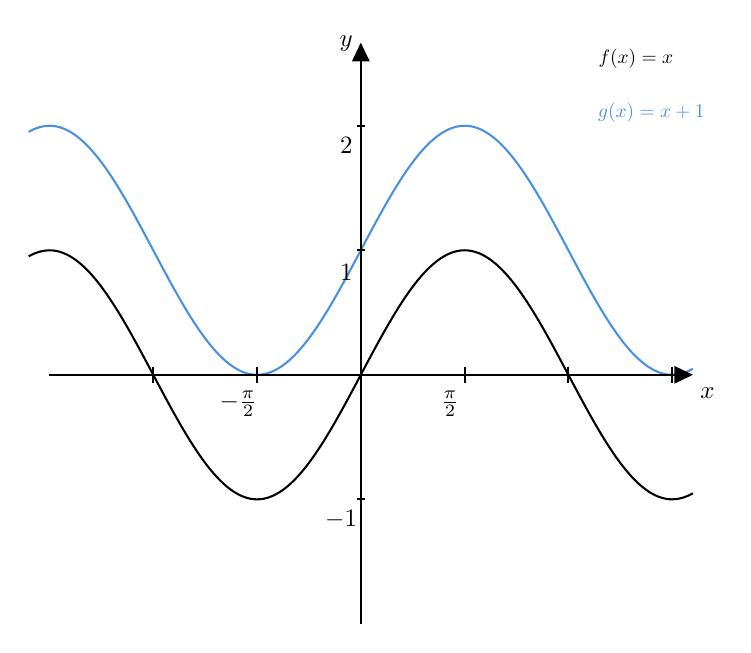
\begin{tikzpicture}[x=0.75pt,y=0.75pt,yscale=-1,xscale=1]
%uncomment if require: \path (0,300); %set diagram left start at 0, and has height of 300

%Shape: Wave [id:dp94416819522044] 
\draw   (180,102.94) .. controls (183.26,101.04) and (186.58,100) .. (190,100) .. controls (208.1,100) and (223.69,129.26) .. (240,160) .. controls (256.31,190.74) and (271.9,220) .. (290,220) .. controls (308.1,220) and (323.69,190.74) .. (340,160) .. controls (356.31,129.26) and (371.9,100) .. (390,100) .. controls (408.1,100) and (423.69,129.26) .. (440,160) .. controls (456.31,190.74) and (471.9,220) .. (490,220) .. controls (493.42,220) and (496.74,218.96) .. (500,217.06) ;
%Shape: Wave [id:dp05495114548578883] 
\draw  [color={rgb, 255:red, 74; green, 144; blue, 226 }  ,draw opacity=1 ] (180,42.94) .. controls (183.26,41.04) and (186.58,40) .. (190,40) .. controls (208.1,40) and (223.69,69.26) .. (240,100) .. controls (256.31,130.74) and (271.9,160) .. (290,160) .. controls (308.1,160) and (323.69,130.74) .. (340,100) .. controls (356.31,69.26) and (371.9,40) .. (390,40) .. controls (408.1,40) and (423.69,69.26) .. (440,100) .. controls (456.31,130.74) and (471.9,160) .. (490,160) .. controls (493.42,160) and (496.74,158.96) .. (500,157.06) ;
%Straight Lines [id:da13690129851328403] 
\draw    (190,160) -- (498,160) (240,156) -- (240,164)(290,156) -- (290,164)(340,156) -- (340,164)(390,156) -- (390,164)(440,156) -- (440,164)(490,156) -- (490,164) ;
\draw [shift={(500,160)}, rotate = 180] [fill={rgb, 255:red, 0; green, 0; blue, 0 }  ][line width=0.75]  [draw opacity=0] (8.93,-4.29) -- (0,0) -- (8.93,4.29) -- cycle    ;

%Straight Lines [id:da021329477973490496] 
\draw    (340,280) -- (340,2) (338,220) -- (342,220)(338,160) -- (342,160)(338,100) -- (342,100)(338,40) -- (342,40) ;
\draw [shift={(340,0)}, rotate = 450] [fill={rgb, 255:red, 0; green, 0; blue, 0 }  ][line width=0.75]  [draw opacity=0] (8.93,-4.29) -- (0,0) -- (8.93,4.29) -- cycle    ;


% Text Node
\draw (472.5,7.5) node [scale=0.7]  {$f( x) =\sen x$};
% Text Node
\draw (383,174) node [scale=0.9,color={rgb, 255:red, 0; green, 0; blue, 0 }  ,opacity=1 ]  {$\frac{\pi }{2}$};
% Text Node
\draw (281,174) node [scale=0.9,color={rgb, 255:red, 0; green, 0; blue, 0 }  ,opacity=1 ]  {$-\frac{\pi }{2}$};
% Text Node
\draw (333,110.5) node [scale=0.9]  {$1$};
% Text Node
\draw (330.5,229.5) node [scale=0.9]  {$-1$};
% Text Node
\draw (480,33.5) node [scale=0.7,color={rgb, 255:red, 74; green, 144; blue, 226 }  ,opacity=1 ]  {$g( x) =\sen x+1$};
% Text Node
\draw (507,169) node [scale=0.9]  {$x$};
% Text Node
\draw (333,0.5) node [scale=0.9]  {$y$};
% Text Node
\draw (333,49.5) node [scale=0.9]  {$2$};


\end{tikzpicture}

    \caption{Gráfico da função $g$.}
    \label{img:grafico-translacao-exemplo-g}
  \end{figure}
%
\noindent Uma vez que $g(x) = f(x)+1$ e $1>0$, o gráfico de $g$ é obtível transladando o gráfico de $f$ 1 unidade para cima.

Na Imagem~\ref{img:grafico-translacao-exemplo-h}, é mostrado o gráfico de $g$.
%
  \begin{figure}
    \centering
    

\tikzset{every picture/.style={line width=0.75pt}} %set default line width to 0.75pt        

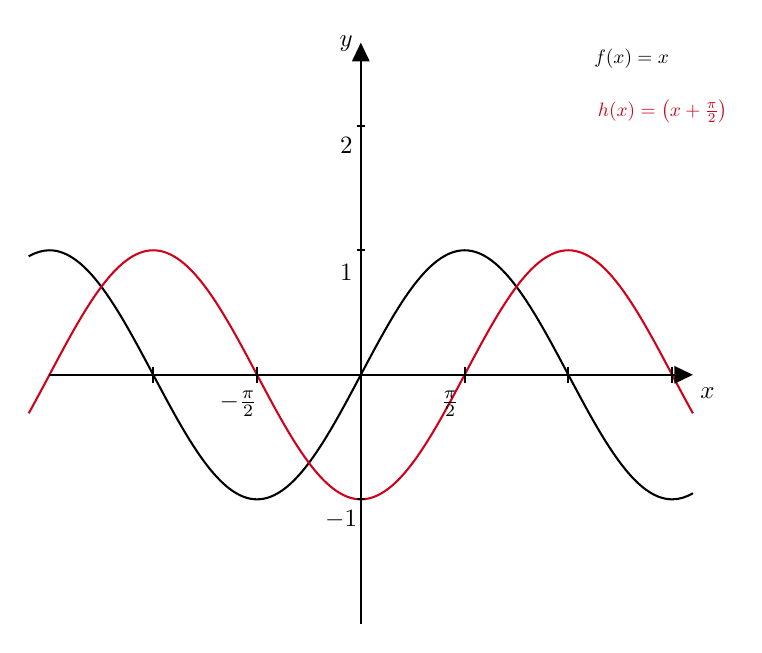
\begin{tikzpicture}[x=0.75pt,y=0.75pt,yscale=-1,xscale=1]
%uncomment if require: \path (0,328); %set diagram left start at 0, and has height of 328

%Shape: Wave [id:dp94416819522044] 
\draw   (180,122.94) .. controls (183.26,121.04) and (186.58,120) .. (190,120) .. controls (208.1,120) and (223.69,149.26) .. (240,180) .. controls (256.31,210.74) and (271.9,240) .. (290,240) .. controls (308.1,240) and (323.69,210.74) .. (340,180) .. controls (356.31,149.26) and (371.9,120) .. (390,120) .. controls (408.1,120) and (423.69,149.26) .. (440,180) .. controls (456.31,210.74) and (471.9,240) .. (490,240) .. controls (493.42,240) and (496.74,238.96) .. (500,237.06) ;
%Shape: Wave [id:dp05495114548578883] 
\draw  [color={rgb, 255:red, 208; green, 2; blue, 27 }  ,draw opacity=1 ] (180,198.54) .. controls (183.32,192.58) and (186.65,186.32) .. (190,180) .. controls (206.31,149.26) and (221.9,120) .. (240,120) .. controls (258.1,120) and (273.69,149.26) .. (290,180) .. controls (306.31,210.74) and (321.9,240) .. (340,240) .. controls (358.1,240) and (373.69,210.74) .. (390,180) .. controls (406.31,149.26) and (421.9,120) .. (440,120) .. controls (458.1,120) and (473.69,149.26) .. (490,180) .. controls (493.35,186.32) and (496.68,192.58) .. (500,198.54) ;
%Straight Lines [id:da13690129851328403] 
\draw    (190,180) -- (498,180) (240,176) -- (240,184)(290,176) -- (290,184)(340,176) -- (340,184)(390,176) -- (390,184)(440,176) -- (440,184)(490,176) -- (490,184) ;
\draw [shift={(500,180)}, rotate = 180] [fill={rgb, 255:red, 0; green, 0; blue, 0 }  ][line width=0.75]  [draw opacity=0] (8.93,-4.29) -- (0,0) -- (8.93,4.29) -- cycle    ;

%Straight Lines [id:da021329477973490496] 
\draw    (340,300) -- (340,22) (338,240) -- (342,240)(338,180) -- (342,180)(338,120) -- (342,120)(338,60) -- (342,60) ;
\draw [shift={(340,20)}, rotate = 450] [fill={rgb, 255:red, 0; green, 0; blue, 0 }  ][line width=0.75]  [draw opacity=0] (8.93,-4.29) -- (0,0) -- (8.93,4.29) -- cycle    ;


% Text Node
\draw (470.5,27.5) node [scale=0.7]  {$f( x) =\sen x$};
% Text Node
\draw (383,194) node [scale=0.9,color={rgb, 255:red, 0; green, 0; blue, 0 }  ,opacity=1 ]  {$\frac{\pi }{2}$};
% Text Node
\draw (281,194) node [scale=0.9,color={rgb, 255:red, 0; green, 0; blue, 0 }  ,opacity=1 ]  {$-\frac{\pi }{2}$};
% Text Node
\draw (333,130.5) node [scale=0.9]  {$1$};
% Text Node
\draw (330.5,249.5) node [scale=0.9]  {$-1$};
% Text Node
\draw (485.5,53) node [scale=0.7,color={rgb, 255:red, 208; green, 2; blue, 27 }  ,opacity=1 ]  {$h( x) =\sen \left( x+\frac{\pi }{2}\right)$};
% Text Node
\draw (507,189) node [scale=0.9]  {$x$};
% Text Node
\draw (333,20.5) node [scale=0.9]  {$y$};
% Text Node
\draw (333,69.5) node [scale=0.9]  {$2$};


\end{tikzpicture}

    \caption{Gráfico da função $h$.}
    \label{img:grafico-translacao-exemplo-h}
  \end{figure}
%
\noindent Uma vez que $h(x) = f\prn{x+\frac {\pi} 2}$ e $\frac {\pi} 2>0$, o gráfico de $h$ é obtível transladando o gráfico de $f$ $\frac {\pi} 2$ unidades para a esquerda.
\end{solution}    